\documentclass[tikz, border=3pt]{standalone}

\usepackage{amsmath,amssymb}
\usepackage{pgfplots}
\pgfplotsset{compat=1.18}
\usepgfplotslibrary{groupplots}
\usetikzlibrary{arrows.meta}
\usepackage{xcolor}

\definecolor{utnblue}{RGB}{0, 51, 102}

\begin{document}
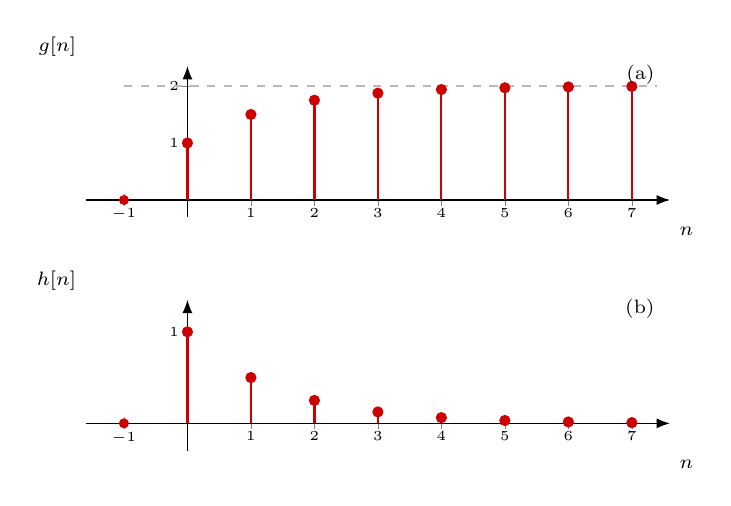
\begin{tikzpicture}[>=Latex, font=\scriptsize]
    \begin{groupplot}[
        group style={group size=1 by 2, vertical sep=1.05cm},
        width=9cm, height=3.5cm,
        axis lines=middle,
        axis line style={->, thin, black},
        xmin=-1.6, xmax=7.6, ymin=-0.3, ymax=2.35,
        xtick={-1,1,2,3,4,5,6,7}, ytick={1,2},
        xlabel={$n$},
        xlabel style={anchor=north west, at={(axis description cs:1,0)}, font=\scriptsize},
        ylabel style={rotate=0, anchor=south east, at={(axis description cs:0,1)}, font=\scriptsize},
        every tick label/.style={font=\tiny, fill=white, inner sep=0.8pt},
        title style={font=\scriptsize, at={(axis description cs:1,1)},
                     anchor=north east, xshift=-2pt, yshift=-2pt},
        clip=false,
    ]
        \nextgroupplot[title={(a)}, ylabel={$g[n]$}]
            \draw[gray!55, dashed, thin] (axis cs:-1,2) -- (axis cs:7.4,2);
            \addplot[ycomb, mark=*, mark size=1.6pt, thick, red!80!black]
                coordinates {(0,1) (1,1.5) (2,1.75) (3,1.875) (4,1.9375)
                             (5,1.96875) (6,1.984375) (7,1.9921875)};
            \addplot[only marks, mark=*, mark size=1.6pt, red!80!black]
                coordinates {(-1,0)};
        \nextgroupplot[title={(b)}, ylabel={$h[n]$}, ymax=1.35, ytick={1}]
            \addplot[ycomb, mark=*, mark size=1.6pt, thick, red!80!black]
                coordinates {(0,1) (1,0.5) (2,0.25) (3,0.125) (4,0.0625)
                             (5,0.03125) (6,0.015625) (7,0.0078125)};
            \addplot[only marks, mark=*, mark size=1.6pt, red!80!black]
                coordinates {(-1,0)};
    \end{groupplot}
\end{tikzpicture}
\end{document}
